\documentclass[11pt,a4paper]{article}
\usepackage{amsmath}
\usepackage{amssymb}
\usepackage{graphicx}
\usepackage{subfigure}
\usepackage{float}
\usepackage{xeCJK}
\usepackage{geometry}
\geometry{left=2.0cm,right=2.0cm,top=2.0cm,bottom=2.0cm}

\title{Energy transfer in ITG/KBM system}
\author{Guangzhi Ren}
\date{\today}

\begin{document}

\maketitle

\section{model equation}

\begin{equation}
 	\frac{dn}{dt}=a\frac{dn_{eq}}{dr}\nabla_\theta\phi-n_{eq}\nabla_{\parallel}v+\nabla_{\parallel}j+\omega_d(n_{eq}\phi-p_e)+D_n\nabla^2_\perp{n}
\end{equation}

\begin{equation}
	\frac{d\nabla^2_\perp\phi}{dt}=-aT_{eq}(\frac{1}{n}\frac{dn_{eq}}{dr}+\frac{1}{T_{eq}}\frac{dT_{eq}}{dr})\nabla_\theta\nabla^2_\perp\phi+\frac{1}{n_{eq}}\nabla_{\parallel}j-\omega_d(T_i+\frac{T_{eq}}{n_{eq}}n+\frac{p_e}{n_{eq}})+D_U\nabla^4_\perp\phi
\end{equation}

\begin{equation}
\frac{dv}{dt}=-\nabla_\parallel{T_i}-2\frac{T_{eq}}{n_{eq}}\nabla_\parallel{n}-\beta{aT_{eq}}(\frac{2}{n_{eq}}\frac{dn_{eq}}{dr}+\frac{1}{T_{eq}}\frac{dT_{eq}}{dr})\nabla_\theta{A}+D_v\nabla^2_\perp{v}
\end{equation}

\begin{equation}
\beta\frac{\partial{A}}{\partial{t}}=-\nabla_\parallel\phi+\frac{T_{eq}}{n_{eq}}\nabla_\parallel{n}+\beta{aT_{eq}}\frac{1}{n_{eq}}\frac{dn_{eq}}{dr}\nabla_\theta{A}+\sqrt{\frac{\pi}{2}\frac{m_e}{m_i}}|\nabla_{\parallel}|(v-\frac{j}{n_{eq}})-\eta{j}
\end{equation}

\begin{equation}
\frac{dT_i}{dt}=a\frac{\partial{T_{eq}}}{\partial{r}}\nabla_\theta\phi-(\Gamma-1)T_{eq}\nabla_\parallel{v}+T_{eq}\omega_d((\Gamma-1)\phi+(2\Gamma-1)T_i+(\Gamma-1)\frac{T_{eq}}{n_{eq}}n)-(\Gamma-1)\sqrt{\frac{8T_{eq}}{\pi}}|\nabla_\parallel|T_i+D_T\nabla_\perp^2{T_i}
\end{equation}


\section{energy balance equation}

energy in system
\begin{equation}
\begin{aligned}
	&E_k=\frac{1}{2}<|\nabla_\perp\phi|^2>	\\
	&E_m=\frac{1}{2}<\frac{\beta}{n_{eq}}|\nabla_\perp\psi|^2>	\\
	&E_n=\frac{1}{2}<\tau\frac{T_{eq}}{n_{eq}^2}|n|^2>	\\
	&E_v=\frac{1}{2}<{\frac{\tau}{\tau+1}}|v|^2>	\\
	&E_t=\frac{1}{2}<{\frac{\tau}{(\Gamma-1)(\tau+1)T_{eq}}}|T|^2>
\end{aligned}
\end{equation}
where 
\begin{equation}
<f>=\frac{\int{f}dV}{\int{dV}}
=\frac{\int{f}\ rdrd\theta{d\zeta}}{\int\ rdrd\theta{d\zeta}}
\end{equation}
total energy
\begin{equation}
	E_{total}={E_k+E_m+E_n+E_v+E_t} 
\end{equation}
time dependence of energy
\begin{equation}
\frac{d}{dt}E_i=\Gamma_F+\Gamma_Q+\Gamma_C+\Gamma_{LD}+\Gamma_{NL}+\Gamma_{S}
\end{equation}


radial transport items
\begin{equation}
\begin{aligned}
	&\Gamma_{Q,n}=<\tau{a}\frac{T_{eq}}{n_{eq}^2}n\nabla_\theta\phi>+<\beta\tau\frac{T_{eq}}{n_{eq}^2}\frac{\partial{j_0}}{\partial{r}}n\nabla_\theta{A}>	\\
	&\Gamma_{Q,v}=-<\frac{\tau}{\tau+1}\beta{aT_{eq}}(\frac{2}{n_{eq}}\frac{dn_{eq}}{dr}+\frac{1}{T_{eq}}\frac{dT_{eq}}{dr})v\nabla_\theta{A}>	\\
	&\Gamma_{Q,t}=<{\frac{\tau}{(\Gamma-1)(\tau+1)T_{eq}}}a\frac{\partial{T_{eq}}}{\partial{r}}T\nabla_\theta\phi>	\\
	&\Gamma_{Q,k}=<-aT_{eq}(\frac{1}{n}\frac{dn_{eq}}{dr}+\frac{1}{T_{eq}}\frac{dT_{eq}}{dr})\phi\nabla_\theta\nabla^2_\perp\phi>+<\frac{\beta}{n_{eq}}\frac{\partial{j_0}}{\partial{r}}\phi\nabla_\theta{A}>	\\
	&\Gamma_{Q,m}=<\frac{\beta}{n_{eq}}{aT_{eq}}\frac{1}{n_{eq}}\frac{dn_{eq}}{dr}j\nabla_\theta{A}>
\end{aligned}
\end{equation}

parallel transport items
\begin{equation}
\begin{aligned}
&\Gamma_{F,k}=<>
\end{aligned}
\end{equation}

curvature items
\begin{equation}
\begin{aligned}
&\Gamma_{C,k}=<>
\end{aligned}
\end{equation}

landau damping items
\begin{equation}
\begin{aligned}
&D_m=<\frac{1}{n_{eq}}\sqrt{\frac{\pi\tau}{2}\frac{m_e}{m_i}}j\nabla_\parallel|(v-\frac{j}{n_{eq}})> \\
&D_t=-<\frac{\tau}{(\tau+1)T_{eq}}\sqrt{\frac{8T_{eq}}{\pi}}T|\nabla_\parallel|T>
\end{aligned}
\end{equation}

diffusion items
\begin{equation}
\begin{aligned}
	&\Gamma_{S,k}=-D_U<|\nabla^2_\perp\phi|^2>	\\
	&\Gamma_{S,m}=-\frac{1}{n_{eq}}D_m<|j|^2>	\\
	&\Gamma_{S,n}=\tau\frac{T_{eq}}{n_{eq}^2}D_n<|\nabla_\perp{n}|^2>	\\
	&\Gamma_{S,v}=-\frac{\tau}{\tau+1}D_v<|\nabla_\perp{v}|^2>	\\
	&\Gamma_{S,t}=-\frac{\tau}{(\Gamma-1)(\tau+1)T_{eq}}D_t<|\nabla_\perp{T}|^2>
\end{aligned}
\end{equation}

time dependence of energy
\begin{equation}
\frac{\partial}{\partial{t}}E_{total}=\Sigma_i[ {\frac{1}{2}({\Gamma_{Q,i}}+{\Gamma_{C,i}}+{\Gamma_{LD,i}})} +\Gamma_{S,i}]
\end{equation}

%
%\section{turbulence}
%\begin{figure}[H]
%	\centering
%	\subfigure[]{
%		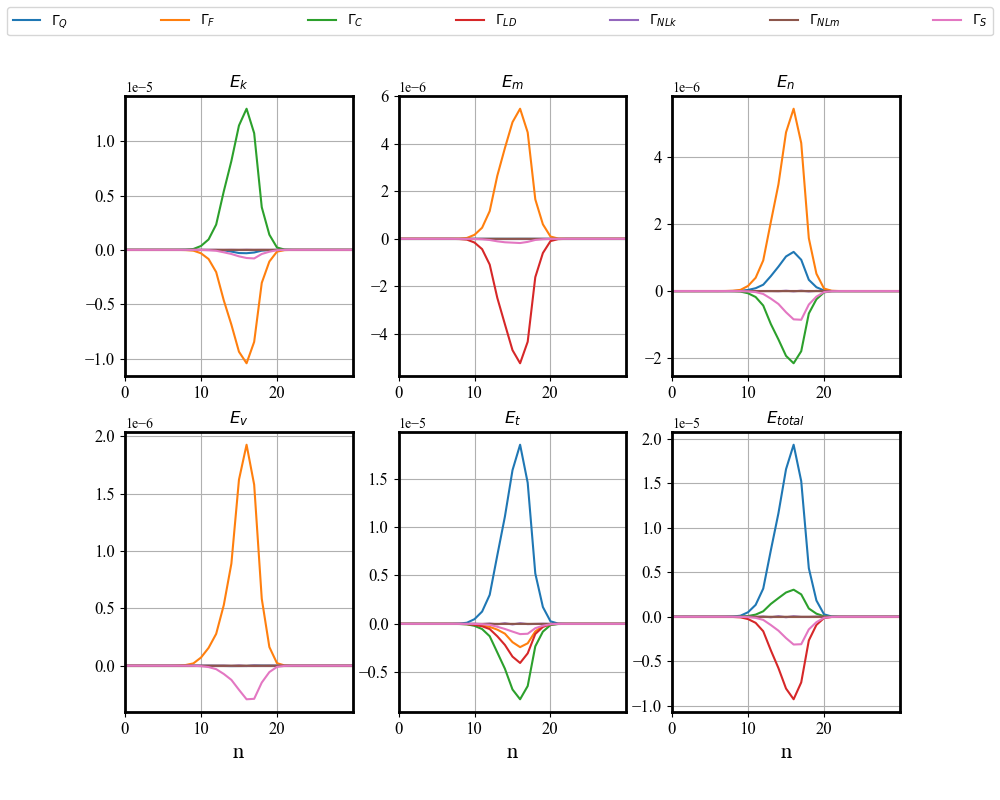
\includegraphics[width=0.45\textwidth]{./images/tur_n_b01_40-80.png} 
%	}
%	\subfigure[]{
%		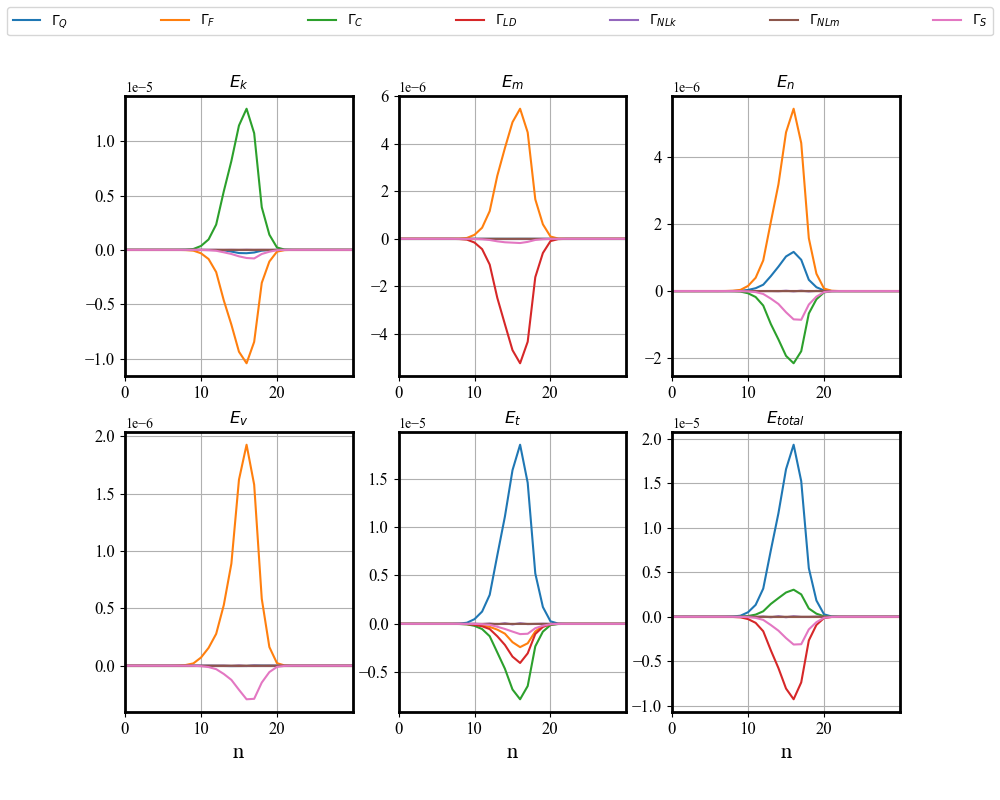
\includegraphics[width=0.45\textwidth]{./images/tur_n_b01_40-80.png}
%	}
%	\caption{(a),(b)}
%\end{figure}
%
%
%\begin{figure}[H]
%	\centering
%	\subfigure[]{
%		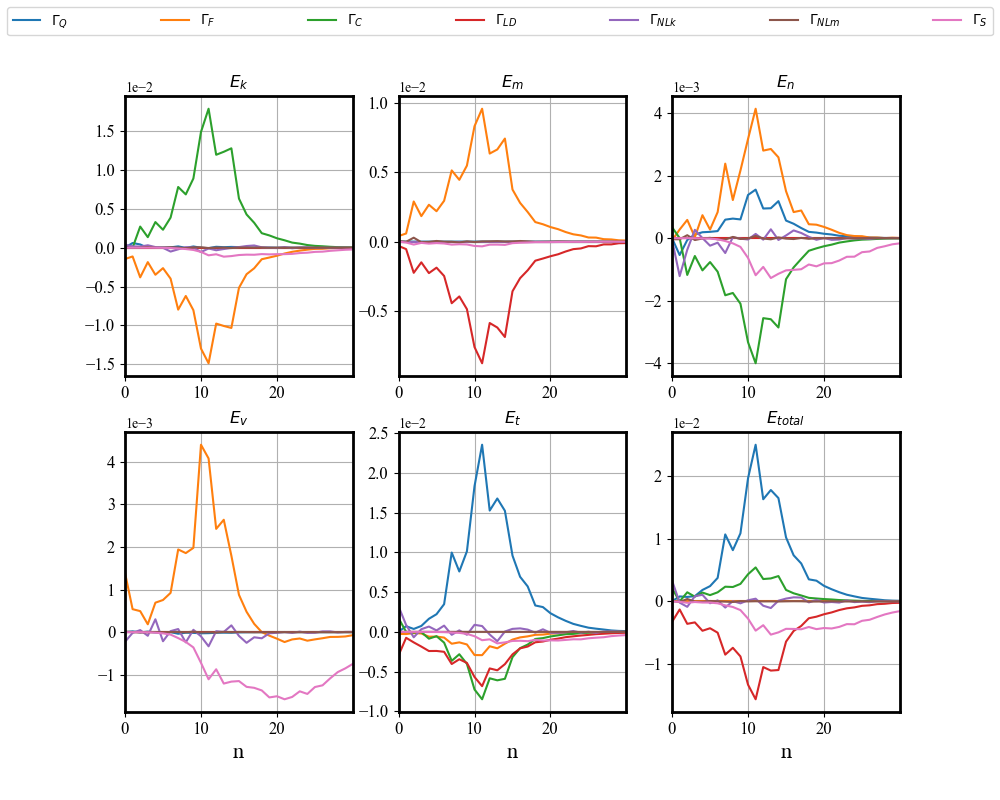
\includegraphics[width=0.45\textwidth]{./images/tur_n_b01_200-250.png} 
%	}
%	\subfigure[]{
%		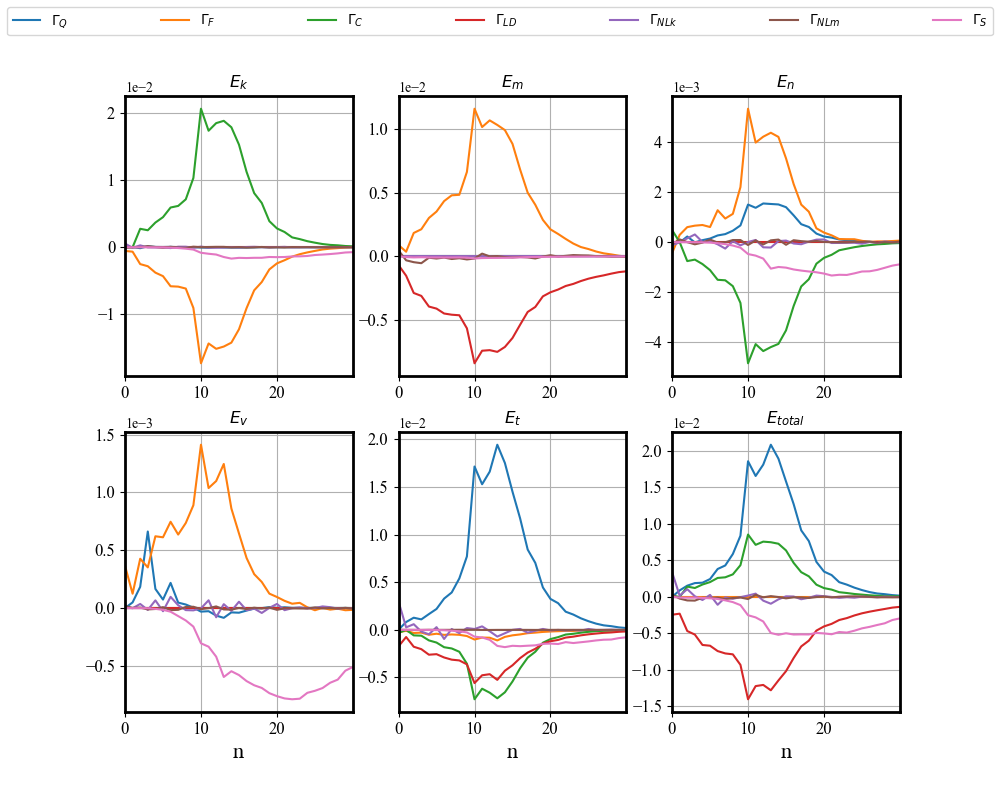
\includegraphics[width=0.45\textwidth]{./images/tur_n_b10_150-250.png}
%	}
%	\caption{(a),(b)}
%\end{figure}
%
%
%\begin{figure}[H]
%	\centering
%	\subfigure[]{
%		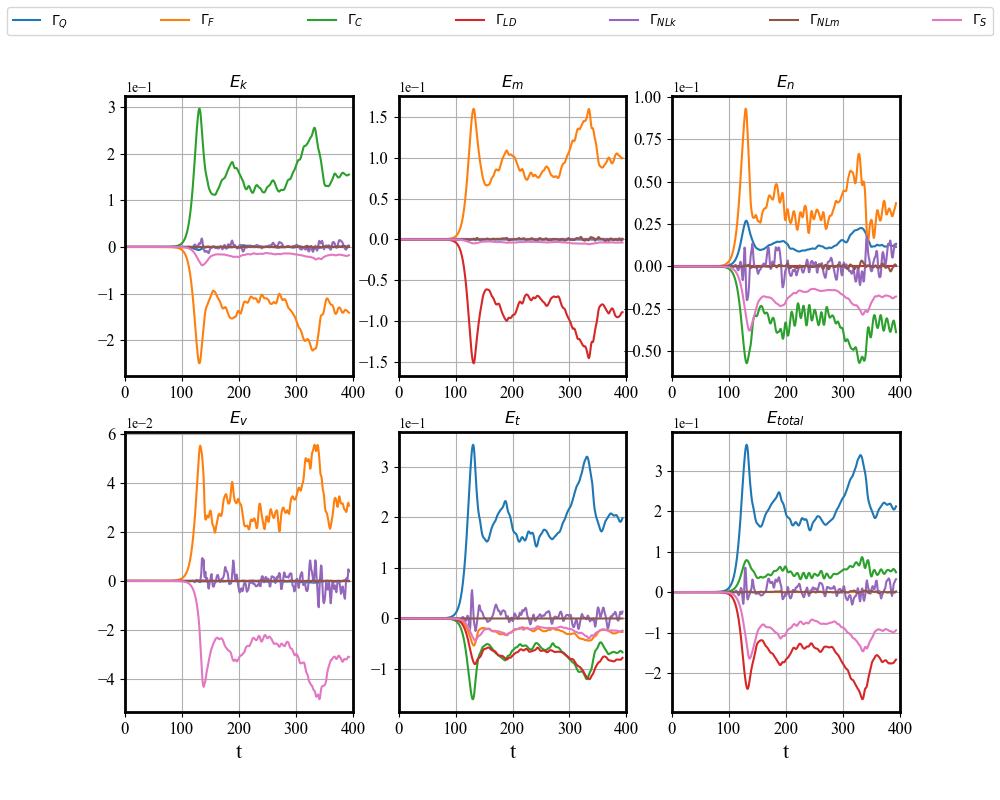
\includegraphics[width=0.45\textwidth]{./images/tur_t_b01.png} 
%	}
%	\subfigure[]{
%		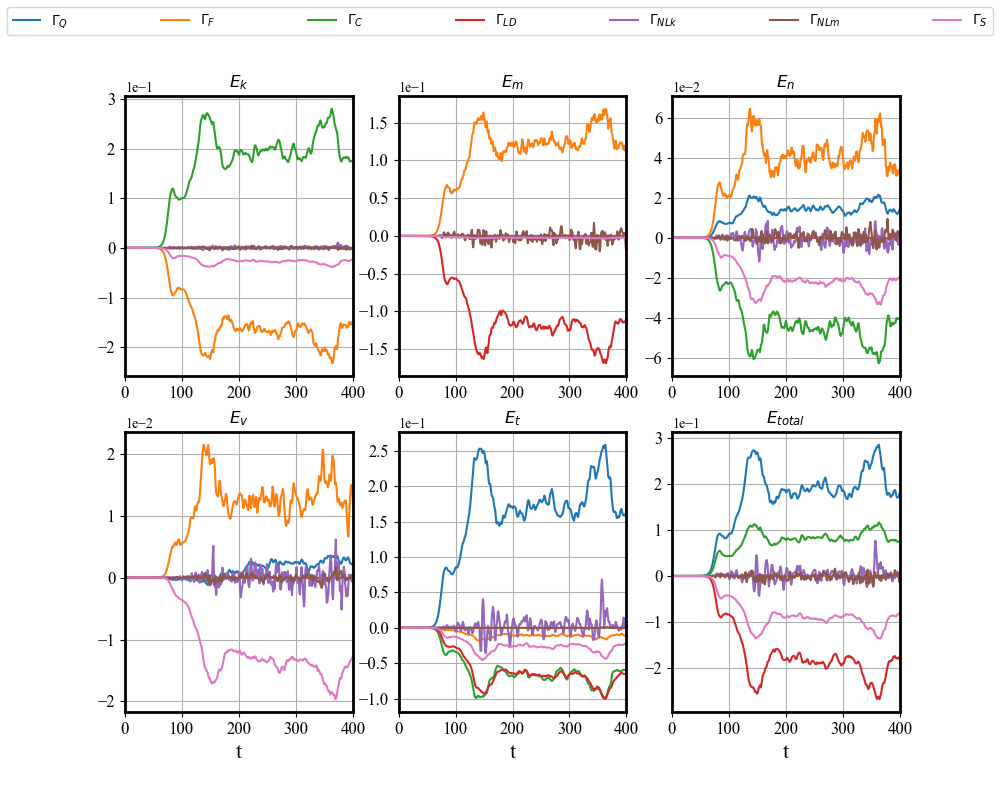
\includegraphics[width=0.45\textwidth]{./images/tur_t_b10.png}
%	}
%	\caption{(a),(b)}
%\end{figure}
%
%
%\begin{figure}[H]
%	\centering
%	\subfigure[]{
%		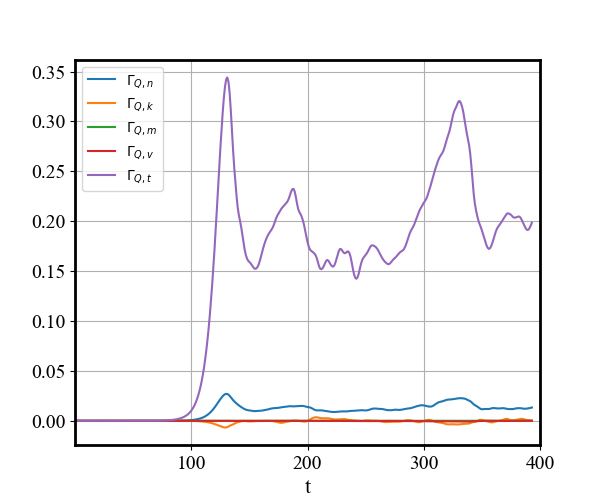
\includegraphics[width=0.45\textwidth]{./images/Q_tur_b01.png} 
%	}
%	\subfigure[]{
%		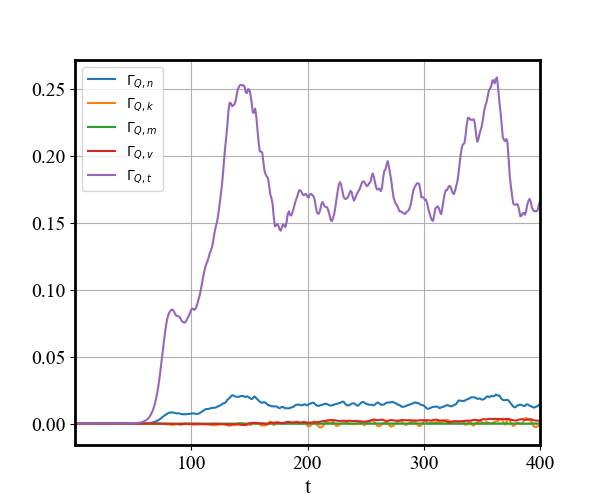
\includegraphics[width=0.45\textwidth]{./images/Q_tur_b10.png}
%	}
%	\caption{(a),(b)}
%\end{figure}
%
%
%
%\section{zonal flow character}
%
%	\begin{figure}[H]
%		\centering
%		\subfigure[]{
%			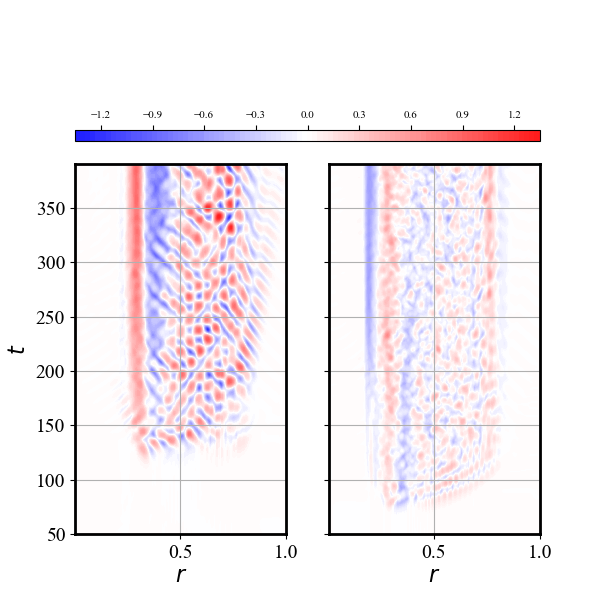
\includegraphics[width=0.35\textwidth]{./images/zf_contour.png} 
%		}
%		\subfigure[]{
%			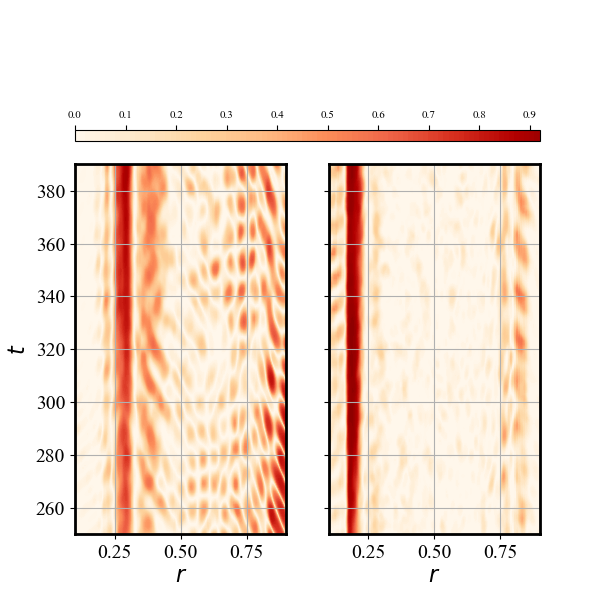
\includegraphics[width=0.35\textwidth]{./images/zf_ratio.png}
%		}
%		\caption{(a)zonal flow as a function of radius and time,(b)$E_{k,ZF}/E_{k,all}$as a function of radius and time}
%	\end{figure}
%
%
%
\section{energy drive of $E_{k,m=0,n=0}$ and $E_{p,m=1,n=0}$}

for zonal flow energy:
\begin{equation}
\frac{\partial}{\partial{t}}E_k=\Gamma_{NLk,k}+\Gamma_{NLm,k}+\Gamma_{C,k}
\end{equation}
for pressure:
\begin{equation}
	p=p_i+p_e=n_0T+(1+\tau)T_0{n}
\end{equation}

\begin{equation}
\frac{\partial}{\partial{t}}E_p=\Gamma_{Q,p}+\Gamma_{F,p}+\Gamma_{C,p}+\Gamma_{LD,p}+\Gamma_{NL,p}+\Gamma_{S,p}
\end{equation}

\begin{equation}
\begin{aligned}
&\Gamma_{Q,p}=<a[(1+\tau)T_{eq}\frac{\partial{n_eq}}{\partial{r}}+n_{eq}\frac{\partial{T_{eq}}}{\partial{r}}]p\nabla_\theta\phi>+<(1+\tau)\beta{T_{eq}}\frac{\partial{j_0}}{\partial{r}}p\nabla_\theta{A}>	\\
&\Gamma_{F,p}=-<(\Gamma+\tau)n_{eq}T_{eq}p\nabla_{\parallel}v>+<(1+\tau)T_{eq}p\nabla_\parallel{j}>	\\
&\Gamma_{LD,p}=-<(\Gamma-1)\sqrt{\frac{8T_{eq}}{\pi}}n_{eq}p|\nabla_\parallel|T>	\\
&\Gamma_{C,p}= <p\omega_d((\Gamma+\tau)n_{eq}T_{eq}\phi)>+<p\omega_d((2\Gamma-1)n_{eq}T_{eq}T)>+<p\omega_d(((\Gamma-1)-\tau(\tau+1))T_{eq}^2n)>	\\
&\Gamma_{NL,p}=	-<p((1+\tau)T_{eq}[\phi,n]+n_{eq}[\phi,T])>
	+<p(\Gamma+\tau)n_{eq}T_{eq}\beta[A,v]>
	-<p(1+\tau)T_{eq}\beta[A,j]>	\\
&\Gamma_{S,p}=	<p[(1+\tau)T_{eq}D_n\nabla_\perp^2n+n_{eq}D_T\nabla_\perp^2{T} ]>	\\
\end{aligned}
\end{equation}
%
%
%\subsection{case of $\beta=0.1\%$}
%
%\begin{figure}[H]
%	\centering
%	\subfigure[]{
%		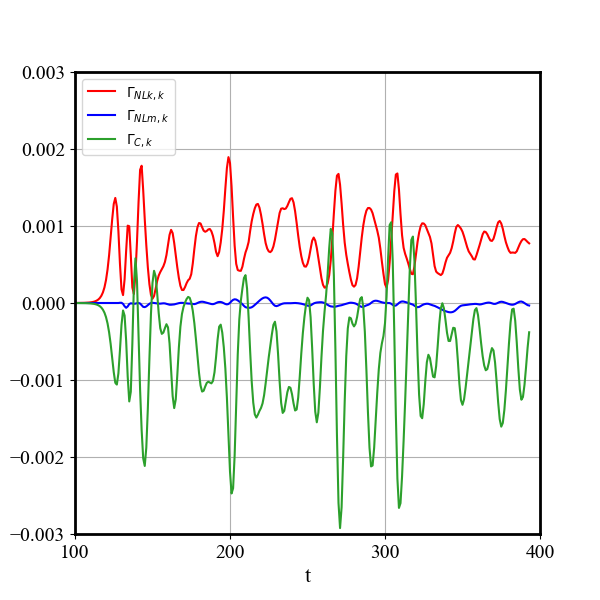
\includegraphics[width=0.35\textwidth]{./images/zf_b01-02-04.png} 
%	}
%	\subfigure[]{
%		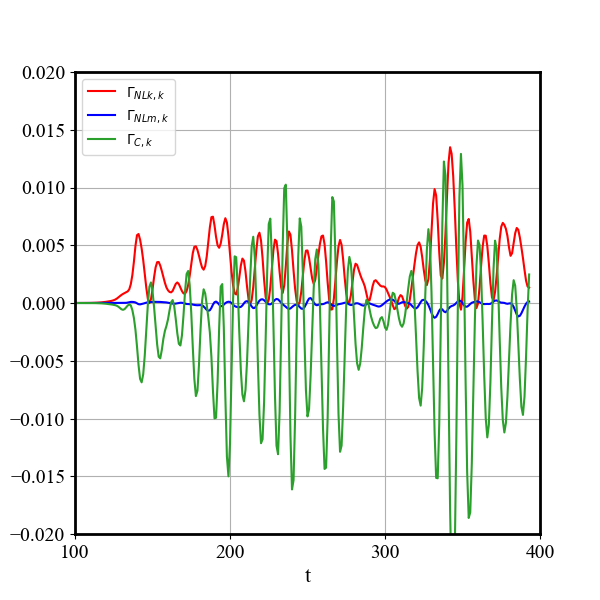
\includegraphics[width=0.35\textwidth]{./images/zf_b01-05-08.png}
%	}
%	\caption{(a),(b)}
%\end{figure}
%
%\begin{figure}[H]
%	\centering
%	\subfigure[]{
%		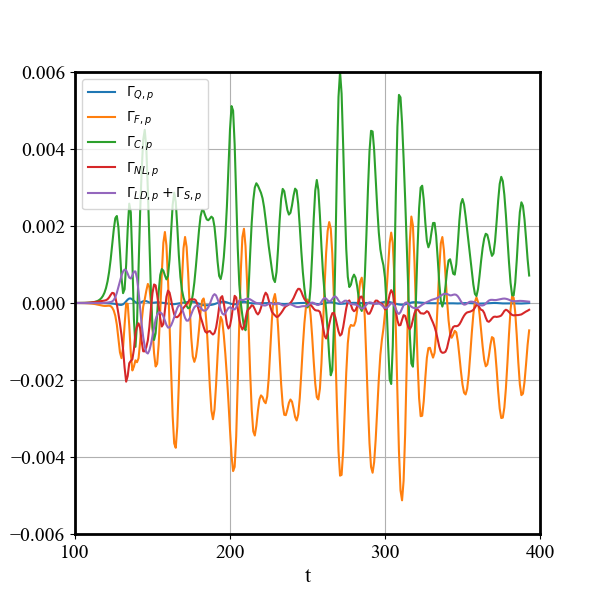
\includegraphics[width=0.35\textwidth]{./images/p10_b01_02-04.png} 
%	}
%	\subfigure[]{
%		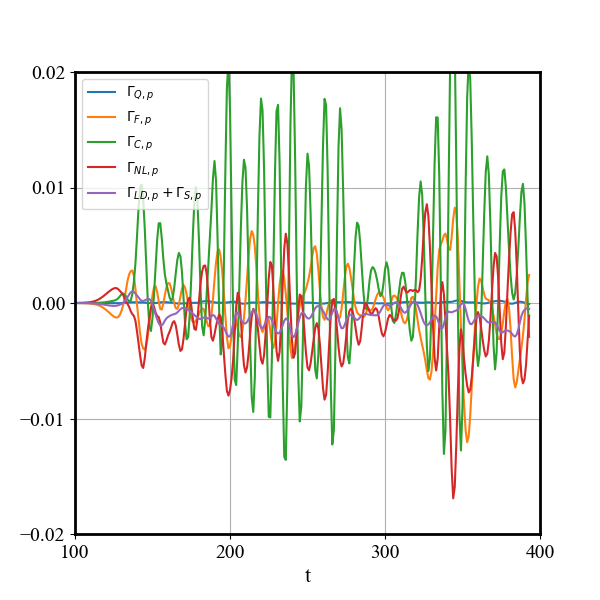
\includegraphics[width=0.35\textwidth]{./images/p10_b01_05-08.png}
%	}
%	\caption{(a),(b)}
%\end{figure}
%
%\begin{figure}[H]
%	\centering
%	\subfigure[]{
%		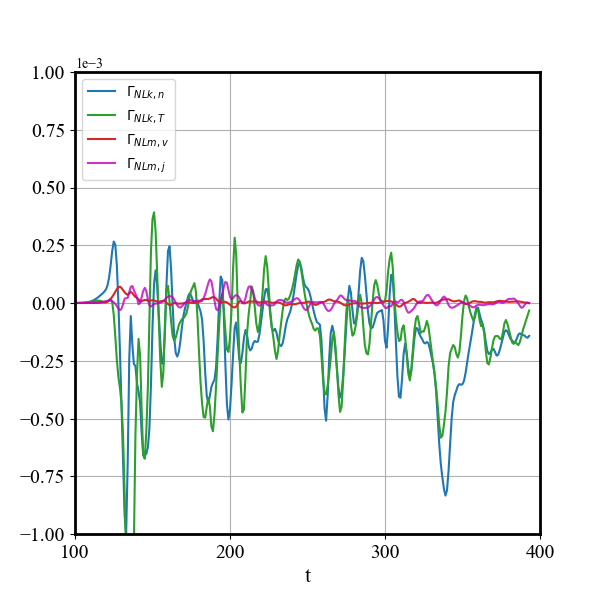
\includegraphics[width=0.35\textwidth]{./images/pnl_b01_02-04.png} 
%	}
%	\subfigure[]{
%		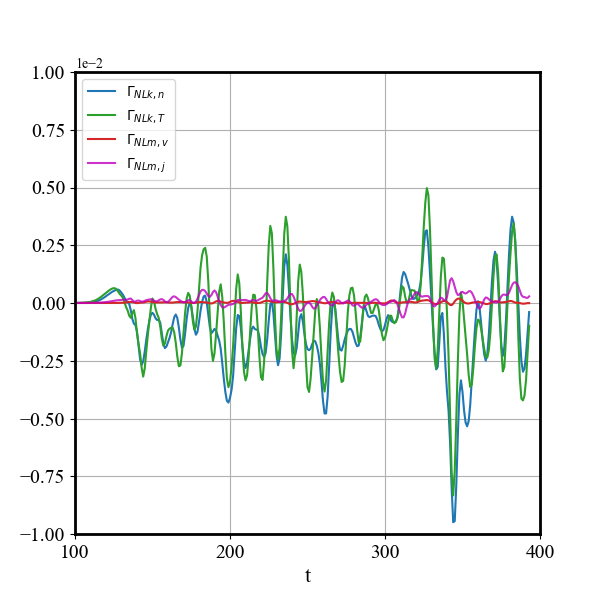
\includegraphics[width=0.35\textwidth]{./images/pnl_b01_05-08.png}
%	}
%	\caption{(a),(b)}
%\end{figure}
%
%\subsection{case of $\beta=1.0\%$}
%
%\begin{figure}[H]
%	\centering
%	\subfigure[]{
%		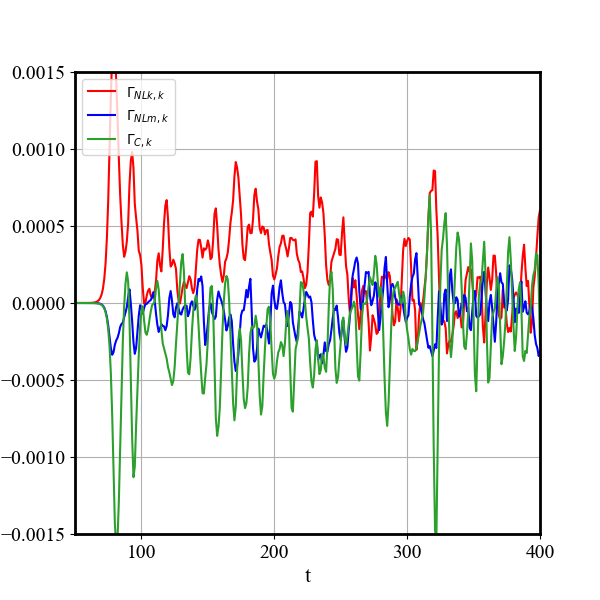
\includegraphics[width=0.35\textwidth]{./images/zf_b10-02-04.png} 
%	}
%	\subfigure[]{
%		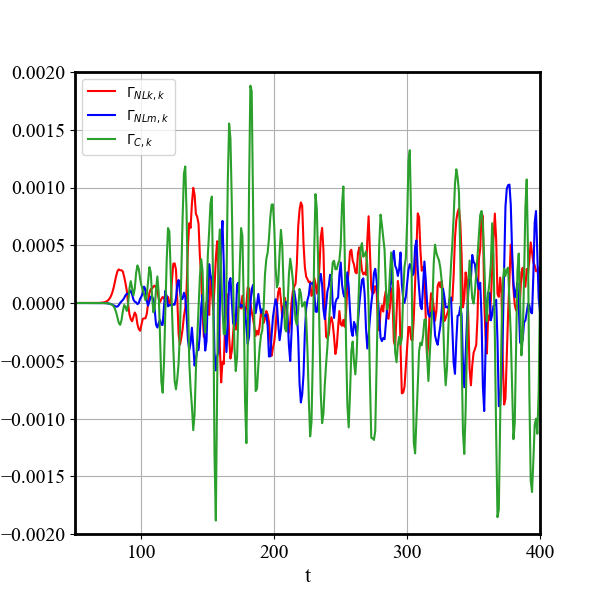
\includegraphics[width=0.35\textwidth]{./images/zf_b10-05-08.png}
%	}
%	\caption{(a),(b)}
%\end{figure}
%
%\begin{figure}[H]
%	\centering
%	\subfigure[]{
%		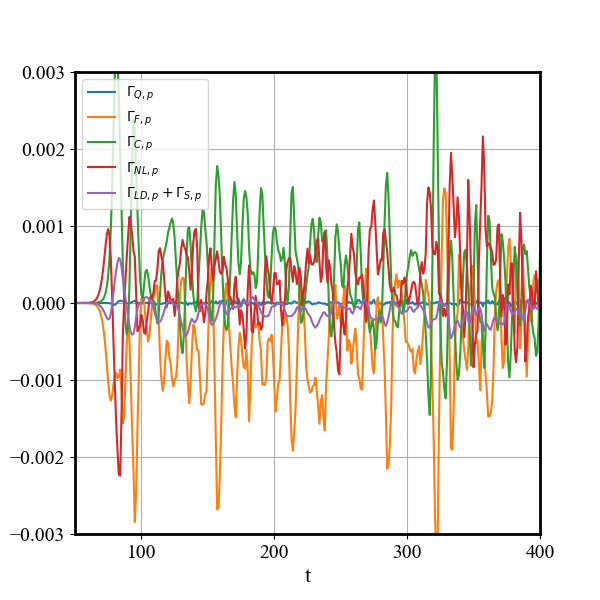
\includegraphics[width=0.35\textwidth]{./images/p10_b10_02-04.png} 
%	}
%	\subfigure[]{
%		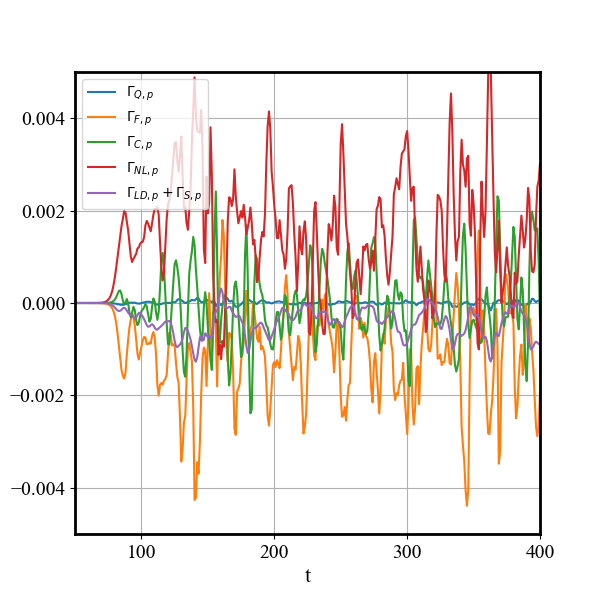
\includegraphics[width=0.35\textwidth]{./images/p10_b10_05-08.png}
%	}
%	\caption{(a),(b)}
%\end{figure}
%
%\begin{figure}[H]
%	\centering
%	\subfigure[]{
%		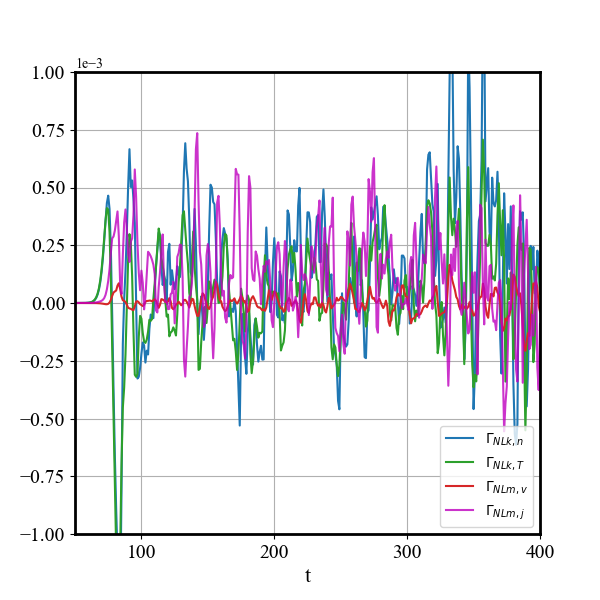
\includegraphics[width=0.35\textwidth]{./images/pnl_b10_02-04.png} 
%	}
%	\subfigure[]{
%		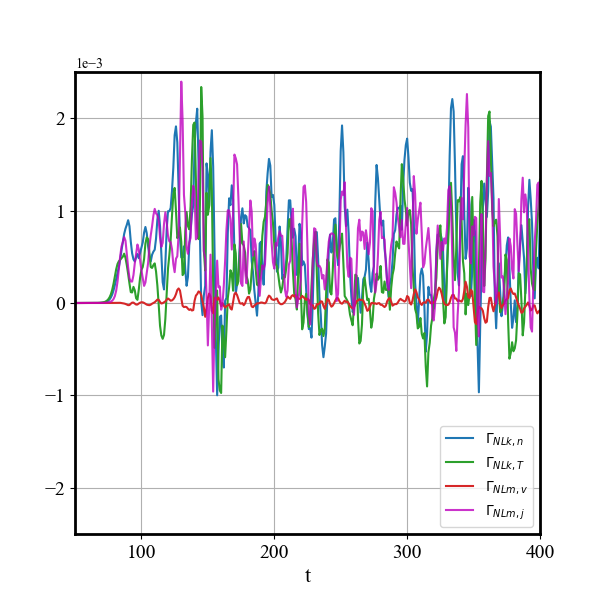
\includegraphics[width=0.35\textwidth]{./images/pnl_b10_05-08.png}
%	}
%	\caption{(a),(b)}
%\end{figure}


\section{Appendix: equation for thr evolution of zonal flow}

	define flux average as 
	\begin{equation}
		<f>=\frac{\int\int\ fd\theta{d\zeta}}{\int\int\ d\theta{d\zeta}}
	\end{equation}
	and the flux-averaged derivation term of vorticity is written as:
	\begin{equation}
	\begin{aligned}
		\frac{\partial}{\partial{t}}<\nabla_\perp^2\phi>
		&=\frac{\partial}{\partial{t}}<\frac{1}{r}\frac{\partial}{\partial{r}}(r\frac{\partial{\phi}}{\partial{r}})>	\\
		&=\frac{1}{r}\frac{\partial}{\partial{r}}r\frac{\partial}{\partial{t}}(\frac{\partial<\phi>}{\partial{r}})	\\
		&=\frac{1}{r}\frac{\partial}{\partial{r}}r\frac{\partial}{\partial{t}}({v_E})
	\end{aligned}
	\end{equation}
	the other flux-averaged term can be written as
	\begin{equation}
		-<[\phi,\Omega]>
		=\frac{1}{r}<\frac{\partial\phi}{\partial\theta}\frac{\partial\Omega}{\partial{r}}-\frac{\partial\phi}{\partial{r}}\frac{\partial\Omega}{\partial\theta}>
	\end{equation}

	\begin{equation}
		<\frac{\partial\phi}{\partial\theta}\frac{\partial\Omega}{\partial{r}}>
		=\int\frac{\partial\phi}{\partial\theta}\frac{\partial\Omega}{\partial{r}}d\theta
		=\int\frac{\partial}{\partial{r}}(\frac{\partial\phi}{\partial\theta}\Omega)d\theta-\int\frac{\partial^2\phi}{\partial{r}\partial\theta}\Omega{d\theta}
	\end{equation}
	
	\begin{equation}
		<\frac{\partial\phi}{\partial{r}}\frac{\partial\Omega}{\partial\theta}>
		=\int\frac{\partial\phi}{\partial{r}}\frac{\partial\Omega}{\partial\theta}d\theta
		=[\Omega\frac{\partial\phi}{\partial{r}}]_0^{2\pi}-\int\frac{\partial^2\phi}{\partial{r}\partial\theta}\Omega{d\theta}
		=-\int\frac{\partial^2\phi}{\partial{r}\partial\theta}\Omega{d\theta}
	\end{equation}
	then:
	\begin{equation}
	\begin{aligned}
		-<[\phi,\Omega]>
		&=\frac{1}{r}\frac{\partial}{\partial{r}}<\Omega\frac{\partial\phi}{\partial\theta}>	\\
		&=\frac{1}{r}\frac{\partial}{\partial{r}}<\phi\frac{\partial\Omega}{\partial\theta}>
	\end{aligned}
	\end{equation}
	and we can convert it to the form like Reynolds stress as follows:
	\begin{equation}
	\begin{aligned}
		\int \frac{\partial\phi}{\partial\theta}\nabla_\perp^2\phi{d\theta}
		&=\int \frac{\partial\phi}{\partial\theta}\frac{1}{r}\frac{\partial}{\partial{r}}r\frac{\partial\phi}{\partial{r}}d\theta+\int \frac{\partial\phi}{\partial\theta}\frac{1}{r^2}\frac{\partial^2\phi}{\partial\theta^2}d\theta	\\
		&=\int \frac{\partial\phi}{\partial\theta}\frac{1}{r}\frac{\partial}{\partial{r}}r\frac{\partial\phi}{\partial{r}}d\theta+\frac{1}{2r^2}\int \frac{\partial}{\partial\theta}(\frac{\partial\phi}{\partial\theta})^2d\theta	\\
		&=\int \frac{\partial\phi}{\partial\theta}\frac{1}{r}\frac{\partial}{\partial{r}}r\frac{\partial\phi}{\partial{r}}d\theta+ \int \frac{1}{r}(r\frac{\partial\phi}{\partial{r}}\frac{\partial^2\phi}{\partial{r}\partial\theta})d\theta	\\
		&=\int \frac{1}{r}\frac{\partial}{\partial{r}}(r\frac{\partial\phi}{\partial{r}}\frac{\partial\phi}{\partial\theta})d\theta	\\
		&=\frac{1}{r}\frac{\partial}{\partial{r}}<r\frac{\partial\phi}{\partial{r}}\frac{\partial\phi}{\partial\theta}>	\\
		&=-\frac{1}{r}\frac{\partial}{\partial{r}}r^2<v_\theta{v_r}>
	\end{aligned}
	\end{equation} 
	and we can deduce the maxwell stress in a similiar way:
	\begin{equation}
	\begin{aligned}
		-\frac{\beta}{n_{eq}}<[A,j]>
		&=\frac{\beta}{n_{eq}}<[A,\nabla_\perp^2{A}]>	\\
		&=\frac{\beta}{n_{eq}}\frac{1}{r}\frac{\partial}{\partial{r}}<j\frac{\partial{A}}{\partial\theta}>	\\
		&=\frac{\beta}{n_{eq}}\frac{1}{r}\frac{\partial}{\partial{r}}<A\frac{\partial{j}}{\partial\theta}>	\\
		&=\frac{\beta}{n_{eq}}\frac{1}{r}\frac{\partial}{\partial{r}}r^2<B_\theta{B_r}>
	\end{aligned}
	\end{equation}

	as for curvature terms,
	\begin{equation}
	\begin{aligned}
		-<\omega_d\cdot{f}>
		&=-2\epsilon<[r\cos\theta,f]>	\\
		&=2\epsilon<\frac{1}{r}(\frac{\partial(r\cos\theta)}{\partial\theta}\frac{\partial{f}}{\partial{r}}-\frac{\partial(r\cos\theta)}{\partial{r}}\frac{\partial{f}}{\partial\theta})>	\\
		&=\frac{2\epsilon}{r}(-<r\sin\theta\frac{\partial{f}}{\partial{r}}>-<\cos\theta\frac{\partial{f}}{\partial\theta}>)	\\
		&=\frac{2\epsilon}{r}(-<r\sin\theta\frac{\partial{f}}{\partial{r}}>-<f\sin\theta>)	\\
		&=-2\epsilon<(\frac{\partial{f}}{\partial{r}}+\frac{f}{r})\sin\theta>\\
		&=-2\epsilon\frac{1}{r}\frac{\partial}{\partial{r}}r<f\sin\theta>
	\end{aligned}
	\end{equation}
	Here,
	\begin{equation}
		f=T_i+\frac{T_{eq}}{n_{eq}}n+\frac{p_e}{n_{eq}}=\frac{p}{n_{eq}}
	\end{equation} 
	then,
	\begin{equation}
		-<\omega\cdot{\frac{p}{n_{eq}}}>=-\frac{2\epsilon}{n_{eq}}\frac{1}{r}\frac{\partial}{\partial{r}}r<p\sin\theta>
	\end{equation}
	so the evolution of zonal flow in the limit of collisionless situation is as follows,
	\begin{equation}
		\frac{1}{r}\frac{\partial}{\partial{r}}r\frac{\partial}{\partial{t}}({v_E})
		=-\frac{1}{r}\frac{\partial}{\partial{r}}  \frac{1}{r}\frac{\partial}{\partial{r}}r^2<v_\theta{v_r}>
		+\frac{1}{r}\frac{\partial}{\partial{r}} 
		\frac{\beta}{n_{eq}}\frac{1}{r}\frac{\partial}{\partial{r}}r^2<B_\theta{B_r}>
		-\frac{2\epsilon}{n_{eq}}\frac{1}{r}\frac{\partial}{\partial{r}}r<p\sin\theta>
	\end{equation}
	eliminate the commom part, we get,
	\begin{equation}
		\frac{\partial}{\partial{t}}<v_E>
		=-\frac{1}{r^2}\frac{\partial}{\partial{r}}r^2<v_\theta{v_r}>
		+\frac{\beta}{n_{eq}}\frac{1}{r^2}\frac{\partial}{\partial{r}}r^2<B_\theta{B_r}>
		-\frac{2\epsilon}{n_{eq}}<p\sin\theta>
	\end{equation} 
	and in the code, we use the alternative expression,
	\begin{equation}
		\frac{\partial}{\partial{t}}<v_E>
		=\frac{1}{r}<\phi\frac{\partial{\Omega}}{\partial\theta}>
		+\frac{\beta}{n_{eq}}\frac{1}{r}<A\frac{\partial{A}}{\partial\theta}>
		-\frac{2\epsilon}{n_{eq}}<p\sin\theta>
	\end{equation} 
	when we use the Fourier expansion,
	\begin{equation}
		\frac{\partial}{\partial{t}}<v_E>
		=\sum_{m1+m2=0}{\phi_{m1}}{\Omega_{\theta,m2}}
		+\sum_{m1+m2=0}{A_{m1}}{j_{\theta,m2}}
		-\frac{i\epsilon}{n_{eq}}(p_{1,0}-p_{-1,0})
	\end{equation}
	
	\begin{equation}
		<p\sin\theta>=\frac{i}{2}(p_{1,0}-p_{-1,0})
	\end{equation}
	

\section{Appendix: equation for thr evolution of $<p\sin\theta>$}
	we can deduce the evolution of $p$ with the drivative equation of $n$ and $T$,
	\begin{equation}
		\frac{\partial}{\partial{t}}p
		=R_Q+R_F+R_C+R_{NL}+R_{LD}+R_{S}
	\end{equation}
	where,
	\begin{equation}
	\begin{aligned}
	R_Q&=
	a[(1+\tau)T_{eq}\frac{\partial{n_{eq}}}{\partial{r}}+n_{eq}\frac{\partial{T_{eq}}}{\partial{r}}]\nabla_\theta\phi
	+(1+\tau)\beta{T_{eq}}\frac{\partial{j_0}}{\partial{r}}\nabla_\theta{A}	\\
	R_F&=
	-(\Gamma+\tau)n_{eq}T_{eq}\nabla_{\parallel}v
	+(1+\tau)T_{eq}\nabla_\parallel{j}	\\
	R_C&=
	\omega_d((\Gamma+\tau)n_{eq}T_{eq}\phi)
	+\omega_d((2\Gamma-1)n_{eq}T_{eq}T)
	+\omega_d(((\Gamma-1)-\tau(\tau+1))T_{eq}^2n)	\\
	R_{NL}&=
	-(1+\tau)T_{eq}[\phi,n]
	-n_{eq}[\phi,T]
	+(\Gamma+\tau)n_{eq}T_{eq}\beta[A,v]
	-(1+\tau)T_{eq}\beta[A,j]	\\
	R_{LD}&=
	-(\Gamma-1)\sqrt{\frac{8T_{eq}}{\pi}}n_{eq}|\nabla_\parallel|T	\\
	R_{S}&=
	(1+\tau)T_{eq}D_n\nabla_\perp^2n
	+n_{eq}D_T\nabla_\perp^2{T}
	\end{aligned}
	\end{equation}
	
	with,
	\begin{equation}
	\begin{aligned}
		<\nabla_\theta{f}\sin\theta>
		&=\int \frac{1}{r}\frac{\partial{f}}{\partial\theta}\sin\theta{d\theta}\\
		&=-\frac{1}{r}<f\cos\theta>
	\end{aligned}
	\end{equation}

	\begin{equation}
	\begin{aligned}
		<\nabla_\parallel{f}\sin\theta>
		&=\int \frac{a}{R}(f_\theta/q+f_\zeta)\sin\theta{d\theta}{d\zeta}\\
		&\approx-\frac{\epsilon}{q}<f\cos\theta>
	\end{aligned}		
	\end{equation}

	\begin{equation}
	\begin{aligned}
		<(\omega_d\cdot{f})\sin\theta>
		&=2\epsilon<[r\cos\theta,f]\sin\theta>	\\
		&=\frac{2\epsilon}{r}(<\frac{\partial{f}}{\partial\theta}\cos\theta\sin\theta>-<r\frac{\partial{f}}{\partial{r}}sin^2\theta>) \\
		&=\epsilon(<\frac{\partial{f}}{\partial{r}}>
		-<(\frac{2f}{r}+\frac{\partial{f}}{\partial{r}})\cos{2\theta}>)
	\end{aligned}
	\end{equation}
	we can convert the terms form to,
	\begin{equation}
	\begin{aligned}
		<R_Q\sin\theta>&=
		a[(1+\tau)T_{eq}\frac{\partial{n_{eq}}}{\partial{r}}+n_{eq}\frac{\partial{T_{eq}}}{\partial{r}}]<\phi\cos\theta>
		+(1+\tau)\beta{T_{eq}}\frac{\partial{j_0}}{\partial{r}}<A\cos\theta>\\
		<R_F\sin\theta>&=
		(\Gamma+\tau)n_{eq}T_{eq}\frac{\epsilon}{q}<v\cos\theta>
		-(1+\tau)T_{eq}\frac{\epsilon}{q}<j\cos\theta>	\\
		<R_C\sin\theta>&=
		\epsilon(\Gamma+\tau)p_{eq}<v_\theta>
		+\epsilon(2\Gamma-1)p_{eq}<\frac{\partial{T}}{\partial{r}}>
		+\epsilon((\Gamma-1)-\tau(\tau+1))T_{eq}^2<\frac{\partial{n}}{\partial{r}}>	\\
		<R_{LD}\sin\theta>&=
		-(\Gamma-1)\sqrt{\frac{8T_{eq}}{\pi}}n_{eq}\frac{\epsilon}{q}<T\sin\theta>	\\
		<R_{NL}\sin\theta>&=
		-<((1+\tau)T_{eq}[\phi,n]+n_{eq}[\phi,T])\sin\theta>	\\
		&+<(\Gamma+\tau)n_{eq}T_{eq}\beta[A,v]\sin\theta>
		-<(1+\tau)T_{eq}\beta[A,j]\sin\theta>
	\end{aligned}
	\end{equation}
	

\end{document}
